%!TEX root = elastic_3d_sbp.tex
\subsection{The fourth order SBP scheme}\label{sub_section_4_1}
We approximate the elastic wave equations (\ref{coarse_problem}) and (\ref{fine_problem}) by two different fourth order SBP schemes. For spatial discretization, we use a Cartesian mesh with mesh size $h_j^c (h_j^f)$ in the coarse domain $\Omega_c$ (fine domain $\Omega_f$) for direction $j$ with $n_j^c = 1/h_j^c +1 (n_j^f = 1/h_j^f +1), j = 1,2,3$. Suppose $(r^{c,(1)}_{i_1^c}, r^{c,(2)}_{i_2^c}, r^{c,(3)}_{i_3^c}), i_1^c = 1,2,\cdots,n_1^c, i_2^c = 1,2,\cdots,n_2^c,i_3^c=0,1,\cdots,n_3^c+1$ are grid points for domain $\Omega_c$ and   $(r^{f,(1)}_{i_1^f}, r^{f,(2)}_{i_2^f}, r^{f,(3)}_{i_3^f}), i_1^f = 1,2,\cdots,n_1^f, i_2^f = 1,2,\cdots,n_2^f,i_3^f=1,\cdots,n_3^f+1$ are grid points for domain $\Omega_f$. Note that we consider ghost points outside each boundary in direction $3$ for coarse domain $\Omega_c$; but for the fine domain $\Omega_f$, the ghost points are used only for the top surface boundary in direction $3$. Denote 
\[{\bf i}^c = (i_1^c,i_2^c,i_3^c), \ {\bf i}^c_{\Omega^c_b} = (i_1^c,i_2^c,1),\  {\bf i}^c_{\Gamma} = (i_1^c,i_2^c,n_3^c),\]
and
\[ {\bf i}^f = (i_1^f,i_2^f,i_3^f), \ {\bf i}^f_{\Gamma} = (i_1^f,i_2^f,1), \ {\bf i}^f_{\Omega_t^f} = (i_1^f,i_2^f,n_3^f).\]
Then in coarse domain $\Omega_c$, we have 
\begin{multline}\label{coarse_scheme}
\rho_{{\bf i}^c}^c ({\bf u}_{tt}^c)_{{\bf i}^c} = \frac{1}{J_{{\bf i}^c}^c}\Big[G_1^c(N_{11}^c){\bf u}_{{\bf i}^c}^c+G_2^c(N_{22}^c){\bf u}_{{\bf i}^c}^c+\uline{\wt{G}}_3^c(N_{33}^c){\bf u}_{{\bf i}^c}^c
+D_1^c(N_{12}^cD_2^c{\bf u}_{{\bf i}^c}^c)+D_1^c(N_{13}^cD_3^c{\bf u}_{{\bf i}^c}^c)
+\\D_2^c(N_{21}^cD_1^c{\bf u}_{{\bf i}^c}^c)+D_2^c(N_{23}^cD_3^c{\bf u}_{{\bf i}^c}^c)
+D_3^c(N_{31}^cD_1^c{\bf u}_{{\bf i}^c}^c)
+D_3^c(N_{32}^cD_2^c{\bf u}_{{\bf i}^c}^c)\Big] := \uline{\wt{L}}_{h^c} {\bf{u}}^c_{{\bf i}^c},
\end{multline}
For the fine domian $\Omega_f$, we impose
\begin{multline}\label{fine_scheme_2}
\rho_{{\bf i}^f}^f ({\bf u}_{tt}^f)_{{\bf i}^f} =
\frac{1}{J_{{\bf i}^f}^f}\Big[G_1^f(N_{11}^f){\bf u}_{{\bf i}^f}^f+G_2^f(N_{22}^f){\bf u}_{{\bf i}^f}^f+\wt{G}_3^f(N_{33}^f){\bf u}_{{\bf i}^f}^f
+D_1^f(N_{12}^fD_2^f{\bf u}_{{\bf i}^f}^f)+D_1^f(N_{13}^fD_3^f{\bf u}_{{\bf i}^f}^f)
+\\D_2^f(N_{21}^fD_1^f{\bf u}_{{\bf i}^f}^f)+D_2^f(N_{23}^fD_3^f{\bf u}_{{\bf i}^f}^f)
+D_3^f(N_{31}^fD_1^f{\bf u}_{{\bf i}^f}^f)+D_3^f(N_{32}^fD_2^f{\bf u}_{{\bf i}^f}^f)\Big] 
:= \wt{L}_{h^f}{\bf{u}}^f_{{\bf i}^f},
\end{multline}
with $ i_3^f = 2,\cdots,n_3^f$ and
\begin{multline}\label{fine_scheme_1}
\rho_{{\bf i}^f_{\Gamma}}^f ({\bf u}_{tt}^f)_{{\bf i}^f_{\Gamma}} = \frac{1}{J_{{\bf i}^f_{\Gamma}}^f}\Big[G_1^f(N_{11}^f){\bf u}_{{\bf i}_\Gamma^f}^f+G_2^f(N_{22}^f){\bf u}_{{\bf i}_\Gamma^f}^f
+G_3^f(N_{33}^f){\bf u}_{{\bf i}^f_{\Gamma}}^f
+D_1^f(N_{12}^fD_2^f{\bf u}_{{\bf i}^f_{\Gamma}}^f)+D_1^f(N_{13}^fD_3^f{\bf u}_{{\bf i}^f_{\Gamma}}^f)
+\\D_2^f(N_{21}^fD_1^f{\bf u}_{{\bf i}^f_{\Gamma}}^f)+
D_2^f(N_{23}^fD_3^f{\bf u}_{{\bf i}^f_{\Gamma}}^f)
+D_3^f(N_{31}^fD_1^f{\bf u}_{{\bf i}^f_{\Gamma}}^f)
+D_3^f(N_{32}^fD_2^f{\bf u}_{{\bf i}^f_{\Gamma}}^f)+{\bm \eta}_{i^f,j^f}\Big]
:= L_{h^f}{\bf u}^f_{{\bf i}^f_{\Gamma}}+{\bm \eta}_{i^f,j^f}/J^f_{{\bf i}^f_{\Gamma}},
\end{multline}
where
\begin{equation}
{\bm \eta} = \rho^f\big|_{\Gamma}\mathcal{P}\left((\rho^c)^{-1}\uline{\wt{L}}_{h^c} {\bf{u}}^c_{{\bf i}^c}\big|_{\Gamma}\right) - L_{h^f}{\bf u}^f_{{\bf i}^f_{\Gamma}}.
\end{equation}
The stencil in the interpolation operator $\mathcal{P}$ can be easily computed by a Talor series expansion. For example, consider $h_1^c = h_2^c, h_1^f = h_2^f$ and $h_1^f = \frac{1}{2}h_1^c$. Then if  $\mathcal{P}$ is a fourth order interpolation operator in $2D$, we have
\begin{align}\label{interpolation}
\left({\bf u}^f\big|_{\Gamma}\right)_{i_1^f,i_2^f} = \left(\mathcal{P} {\bf u}^c\big|_{\Gamma}\right)_{i_1^f,i_2^f} = \left\{\begin{array}{cc}
({\bf u}^c|_{\Gamma})_{(i_1^f+1)/2,(i_2^f+1)/2}, &(i_1^f,i_2^f) = (\text{odd},\text{odd}),\\
\mathcal{B}^1 ({\bf u}^c|_{\Gamma})_{i_1^f/2,(i_2^f+1)/2}, &(i_1^f,i_2^f) = (\text{even},\text{odd}),\\
\mathcal{B}^2 ({\bf u}^c|_{\Gamma})_{(i_1^f+1)/2,i_2^f/2},& (i_1^f,i_2^f) = (\text{odd},\text{even}),\\
\mathcal{B}^1\mathcal{B}^2 ({\bf u}^c|_{\Gamma})_{i_1^f/2,i_2^f/2}, & (i_1^f,i_2^f) = (\text{even},\text{even}),
\end{array}\right.
\end{align}
where $\mathcal{B}^j, j = 1,2$ are the fourth order interpolation operators in $1$D for the direction $j$.  
\begin{figure}[htbp]
	\centering
	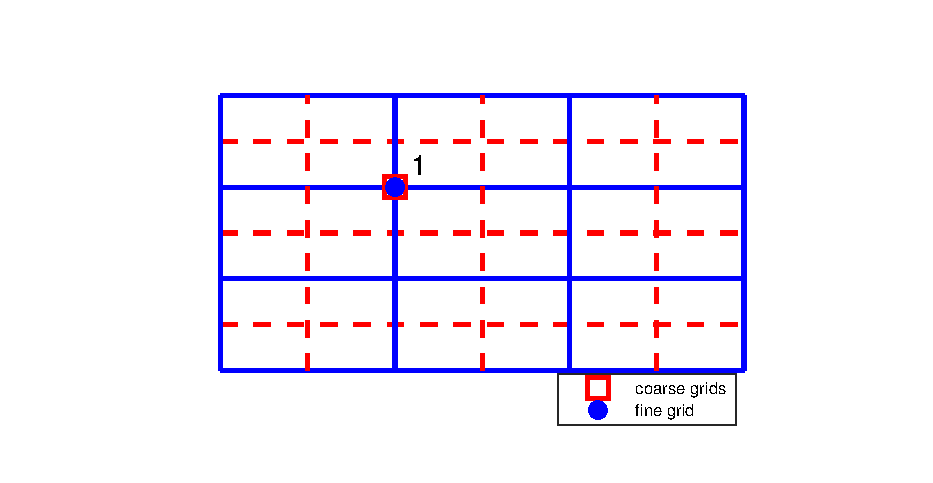
\includegraphics[width=0.45\textwidth]{interpolation1.eps}
	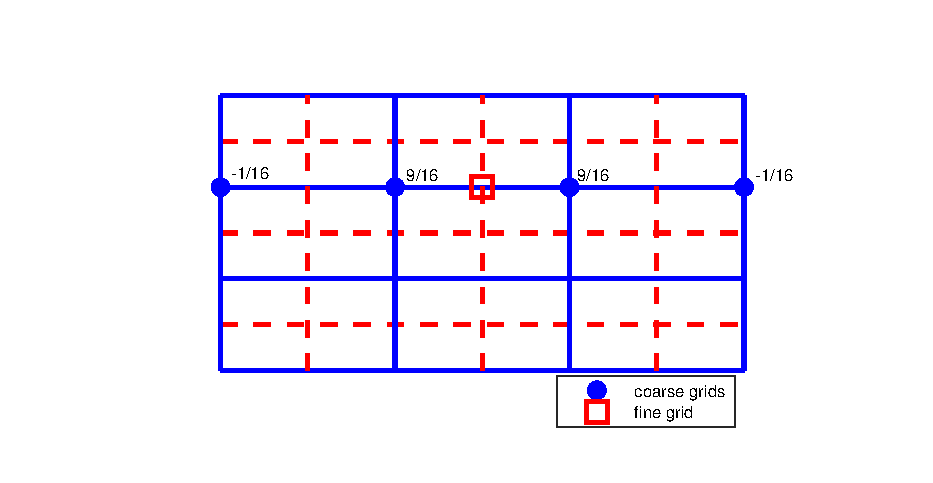
\includegraphics[width=0.45\textwidth]{interpolation2.eps}
	\caption{From left to right, the sketch of interpolation stencil for $(i_1^f,i_2^f) =$ (odd, odd) and $(i_1^f,i_2^f) =$ (even, odd) respectively. The number at the right-top corner are the coefficients of the corresponding coarse grids.}\label{interpolation_1_2}
\end{figure}
Figure \ref{interpolation_1_2} illustrates the interpolation coefficients when $(i_1^f,i_2^f) = $ (odd, odd) and  $(i_1^f,i_2^f) = $ (even, odd) respectively. While Figure \ref{interpolation_3_4} gives the interpolation coefficients when $(i_1^f,i_2^f) = $ (odd, even) and  $(i_1^f,i_2^f) = $ (even, even) respectively.
\begin{figure}[htbp]
	\centering
	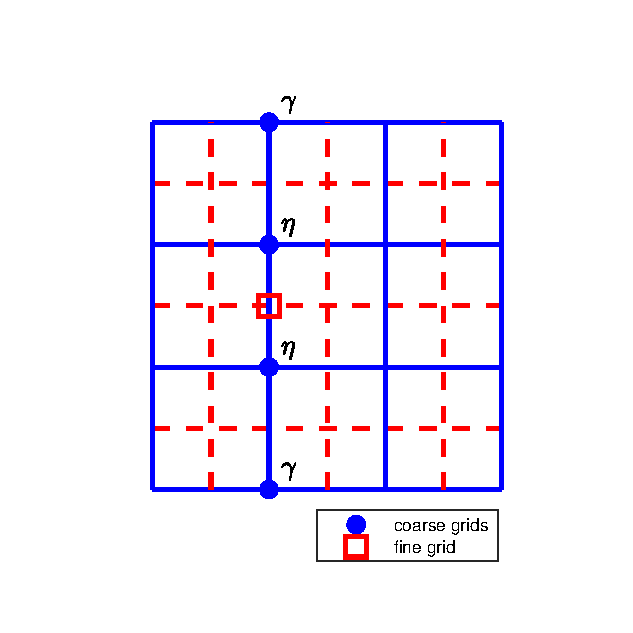
\includegraphics[width=0.45\textwidth]{interpolation3.eps}
	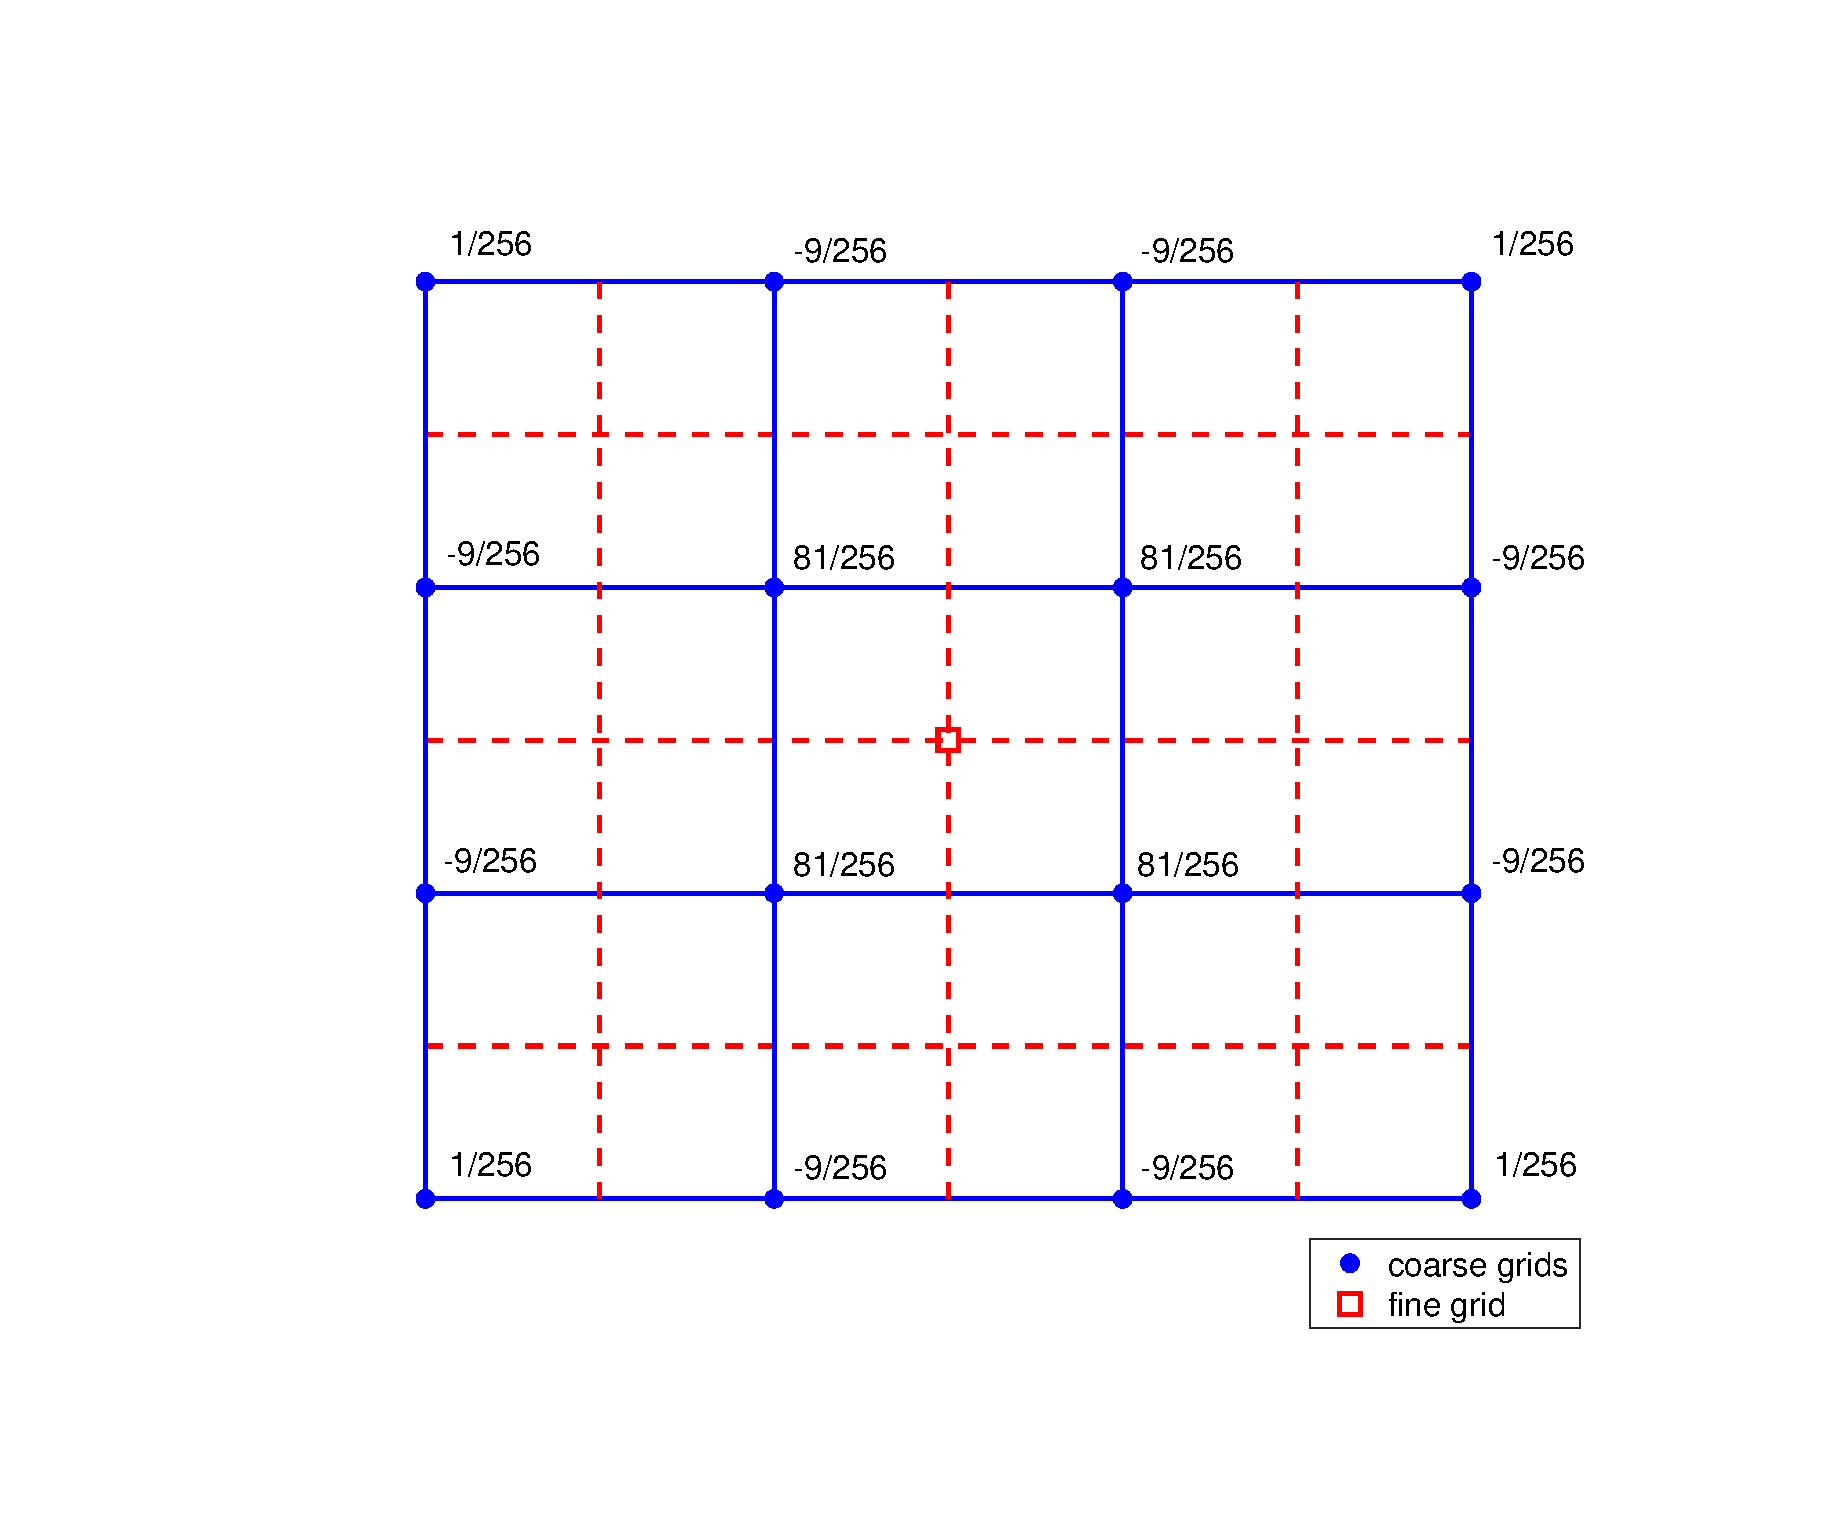
\includegraphics[width=0.45\textwidth]{interpolation4.eps}
	\caption{From left to right, the sketch of interpolation stencil for $(i_1^f,i_2^f) =$ (odd, even) and $(i_1^f,i_2^f) =$ (even, even) respectively. The number at the right-top corner are the coefficients of the corresponding coarse grids.}\label{interpolation_3_4}
\end{figure}

Furthermore, the compatibility condition of the intrpolation operator $\mathcal{P}$ and restriction operator $\mathcal{R}$, $\mathcal{P} = 4\mathcal{R}^T$ for $h_1^c = 2h_1^f$ in $2$D, determines the corresponding restriction operator $\mathcal{R}$ with
\begin{equation}\label{restriction}
({\bf u}^c|_{\Gamma})_{i^c,j^c} = (\mathcal{R}{\bf u}^f|_{\Gamma})_{i^c,j^c} = \mathcal{A}^2\mathcal{A}^1 ({\bf u}^f|_{\Gamma})_{2i^c-1,2j^c-1},
\end{equation}
where $\mathcal{A}^j, j = 1,2$ are the fourth order restriction operators in $1$D for the direction $j$. Figure \ref{extrapolation} shows the restriction coefficients for the coarse grids $(i_1^c,i_2^c)$.

\begin{figure}[htbp]
	\centering
	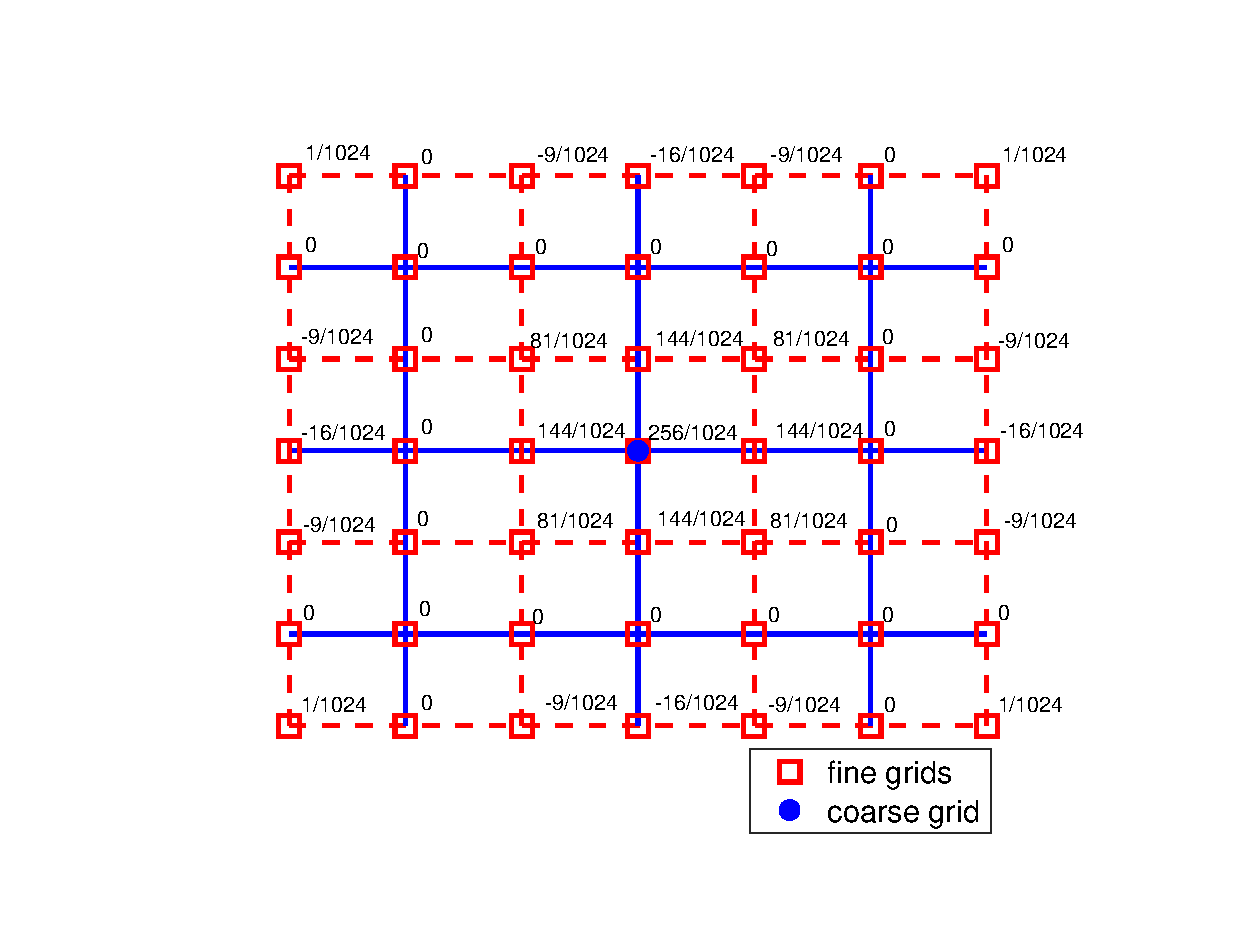
\includegraphics[width=0.8\textwidth]{restriction1.eps}
	\caption{The sketch of restriction operator in $2$D. The number at the right-top corner are the coefficients of the corresponding fine grids.}\label{extrapolation}
\end{figure}
For the simplicity of analysis, we introduce a general notation for the schemes (\ref{fine_scheme_2}) and (\ref{fine_scheme_1}) in the fine domain $\Omega_f$,
\begin{align}\label{fine_scheme}
\rho^f_{{\bf i}^f} ({\bf u}_{tt}^f)_{{\bf i}^f} = \hat{L}_{h^f}{\bf u}^f_{{\bf i}^f} =  \left\{
\begin{aligned}
&\wt{L}_{h^f}{\bf{u}}^f_{{\bf i}^f}, \ \ i_3^f = 2,3,\cdots,n_3^f,\\
&L_{h^f}{\bf u}^f_{{\bf i}^f_{\Gamma}}+{\bm \eta}_{i^f,j^f}/J^f_{{\bf i}^f_{\Gamma}},
\end{aligned}
\right.
\end{align}
For the grids in the fine domain $\Omega^f$  that are lying on the interface $\Gamma$, we impose the continuity of the solution,
\begin{equation}\label{data_continuous_curvi}
{\bf u}^f\big|_{\Gamma} = \mathcal{P}\big({\bf u}^c\big|_{\Gamma}\big).
\end{equation}
As for the ghost points which are close to the top surface of the coarse domian, we impose the continuity of the traction force,
\begin{equation}\label{traction_continuous_curvi}
{\bf n}^c\cdot\mathcal{T}^c \big|_\Gamma = \mathcal{R}\left(-{\bf n}^f\cdot\mathcal{T}^f\big|_\Gamma - \frac{h_3^f\omega_1^{(3)}{\bm \eta}}{J^f\big|\nabla r_f^{(3)}\big|}\Bigg|_\Gamma\right).
\end{equation}